\subsection{$\Kshort$ and $\Lambda$ ($\AntiLa$) reconstruction}
\label{sec:V0Reco}

\begin{table}[t]
\centering
\begin{tabular*}{\linewidth}{@{\extracolsep{\fill}}lr}
\hline
& \\ [-0.7em]
Selection variable & Cut value \\ [0.3em]
\hline
& \\ [-0.7em]
2D decay radius                                    & $>0.50$~cm   \\[0.3em]
Daughter track DCA to prim. vertex                 & $>0.06~$cm   \\[0.3em]
DCA between daughter tracks                        & $<1.0\sigma$ \\[0.3em]
Cosine of pointing angle ($\Kshort$)               & $>0.97$      \\[0.3em]
Cosine of pointing angle ($\Lambda$ and $\AntiLa$) & $>0.995$     \\[0.3em]
Proper lifetime ($\Kshort$)                        & $<20$~cm     \\[0.3em]
Proper lifetime ($\Lambda$ and $\AntiLa$)          & $<30$~cm     \\[0.3em]   
$\Kshort$ mass rejection window ($\Lambda$ and $\AntiLa$) & $\pm 10~\MeVcc$ \\[0.3em]
$\Lambda$ and $\AntiLa$ mass rejection window ($\Kshort$) & $\pm 5~\MeVcc$  \\[0.3em]
\hline
\end{tabular*}
\caption{$\Vzero$ topological selection criteria.}
\label{tab:c05V0cuts}
\end{table}

The $\Vzero$ particles, $\Kshort$ and $\Lambda$ ($\AntiLa$), were identified exploring the characteristics of their weak decay topologies in the channels $\Kshort\to\pi^{+}\pi^{-}$ and $\Lambda(\AntiLa)\to{\rm p}\pi^{-}(\pbar\pi^{-})$, which have branching ratios of $69.2\%$ and $63.9\%$, respectively~\cite{Agashe:2014kda}.
The selection criteria used to define $\Vzero$ candidates are listed in table~\ref{tab:c05V0cuts} (see \cite{Aamodt:2011zza} for details).
The $\Vzero$ decay-product tracks are selected in the acceptance window $\abs{\hlab}<0.8$, only the candidates reconstructed in $\abs{\hlab}<0.75$ are retained to keep $>50\%$ of acceptance and reconstruction efficiency at plateau around $\hlab=0$ \ask{(is it clear or is it needed?)}.
A five-standard-deviation particle-identification cut was applied on the difference between $\dedx$ in the TPC and that defined by parameterized Bethe-Bloch curve for the $\Vzero$ decay-product tracks.
In addition, by using proper lifetime selection coupled to cosine of pointing angle ($\cos\theta_{\rm pointing}$) selection of $\cos\theta_{\rm pointing}>0.995$, a significant amount of secondary $\Lambda$ ($\AntiLa$) generated in detector material are removed.
The residual contamination entering the selections was $<1\%$ and was neglected~\cite{Abelev:2013xaa}.
The yield of $\Vzero$ signal is extracted from the invariant mass, $M_{\rm inv}$, distribution of identified $\Vzero$ candidates subtracting the combinatory background from the peak region with the bin counting method.
The background was determined by fitting first order polynomials to sideband regions.
The signal region and sidebands are defined on the basis of the $\pT$-dependent mass resolution as the windows in $\abs{M_{\rm inv}-M_{0}}<6\sigma$ and $6\sigma<\abs{M_{\rm inv}-M_{0}}<12\sigma$, respectively, where $M_{0}$ and $\sigma$ are the mean and width of invariant mass distribution extracted by the Gaussian fit.

The yield of $\Vzero$s associated to the hard scatterings are tagged by the charged particle jets in $\pT[jet]^{\rm ch}>10~\GeVc$ and $>20~\GeVc$ within the cone $R$ (JC selection) done with the following steps.
\begin{itemize}
\item Selecting $\Vzero$ candidates in $R(\Vzero,{\rm jet})<R$, where,
\begin{equation}
R(\Vzero,{\rm jet})=\sqrt{(\hlab^{\rm jet}-\hlab^{\Vzero})^{2}-(\varphi^{\rm jet}-\varphi^{\Vzero})^{2}}
\end{equation}
is  the distance between the $\Vzero$ candidate and jet axis in pseudo-rapidity and azimuthal angle ($\hlab$--$\varphi$) plane.
\item Extracting the signal yield of selected $\Vzero$s via the bin counting approach.
\end{itemize}
Figure~\ref{fig:c05V0FitInvM} shows the comparison of the $\pT$-dependent mean and width of invariant mass distribution for inclusive $\Vzero$s and JC $\Vzero$s.
The values between these two selections are consistent within statistical uncertainties.
To avoid statistic fluctuations found in JC selection, the yields of JC $\Vzero$s are extracted using the mean and $\sigma$ obtained from the inclusive $\Vzero$s.
It is wealth to notice that, by requiring the DCA to primary vertex in transverse plane $>0.06$~cm sufficiently separates $\Vzero$ decay-product tracks from hybrid tracks, which are constraint to the primary vertex.
The overlapping fraction between them is $\sim 0.1\%$.
The identified $\Vzero$ candidates, therefor, have almost no correlation to jets.


\begin{figure}[htb]
\begin{center}
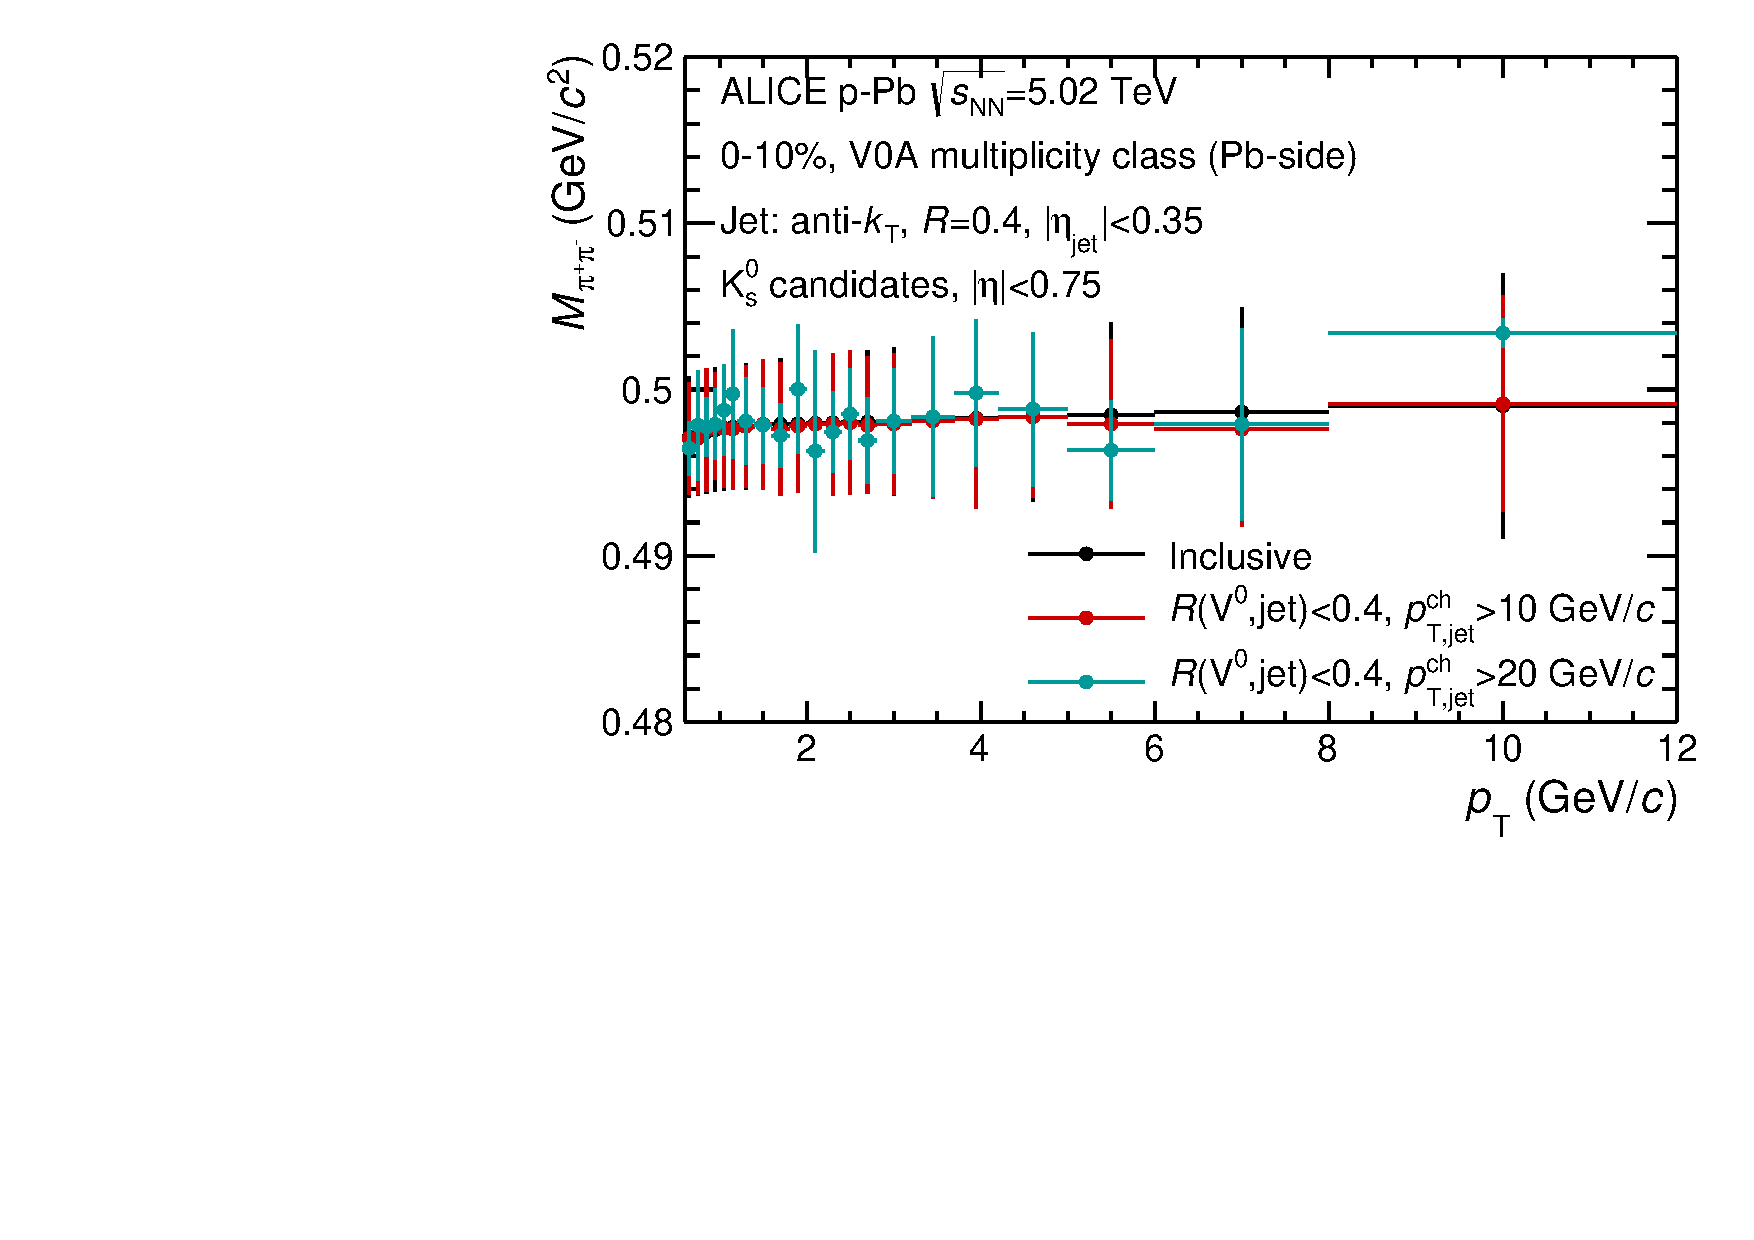
\includegraphics[width=.48\textwidth]{cFitInvM_Kshort}
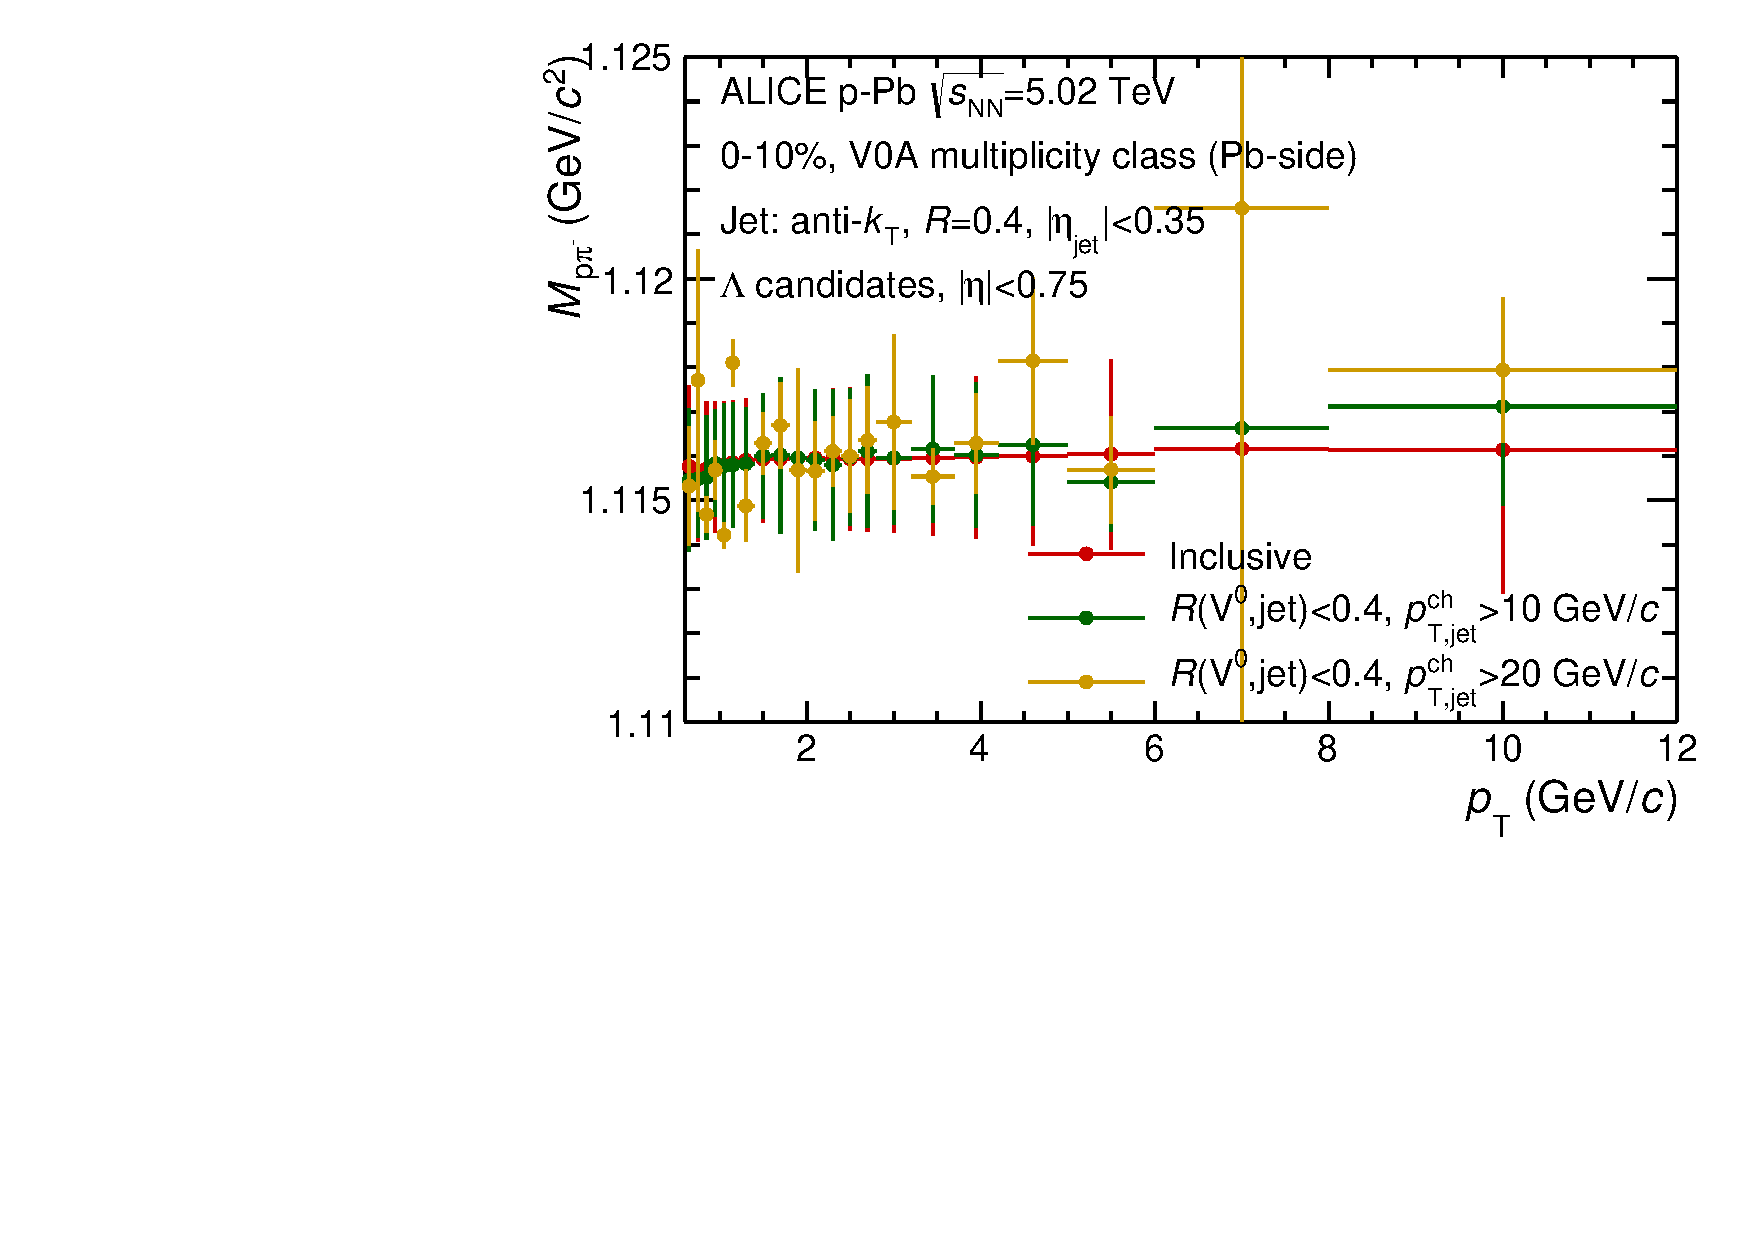
\includegraphics[width=.48\textwidth]{cFitInvM_Lambda}
\caption{The $\pT$-dependent mean of $\Vzero$ invariant mass distribution extracted by the Gaussian fit. The vertical error bar shows the width of the distribution.}
\label{fig:c05V0FitInvM}
\end{center}
\end{figure}

The contribution of $\Xi^{\pm}$ weak decays to the inclusive $\Lambda$ ($\AntiLa$) yield was corrected following a data-driven approach~\cite{Abelev:2013haa} using the measured $\Xi^{\pm}$ spectra as the inputs in a simulation of decay kinematics to evaluate the fraction of feed-down $\Lambda$ ($\AntiLa$).
The contribution from $\Xi^{0}$ decays was taken into account in the same way by assuming $\Xi^{-}(\Xi^{+})/\Xi^{0}=1$~\cite{Abelev:2013haa,Roesler:2000he,Skands:2010ak}.
The feed-down contribution for $\Lambda$ ($\AntiLa$) with JC selection was estimated based on the evaluated feed-down fraction of inclusive $\Lambda$ ($\AntiLa$) at high-$\pT$ and interpolated to the lower $\pT$ using \textsc{Pythia}\,8~\cite{Sjostrand:2007gs} Monte Carlo simulations.
\ask{-- Do we need more details?}

The acceptance and reconstruction efficiency was extracted from a Monte Carlo simulation based on \textsc{Dpmjet}\,3.05 event generator~\cite{Roesler:2000he} and GEANT\,3.21~\cite{Brun:1994aa} transport model for the detector (more details can be found in~\cite{Aamodt:2011zza}).
It has been shown that, the $\pT$ and $\eta$-dependent local efficiencies, $\epsilon(\pT,\eta)$, of $\Vzero$s in different selections are the same \ask{(is there a ref?)}.
To correct the $\pT$-differential yield, the $\pT$-dependent efficiency, $\epsilon(\pT)$, is given by integrating local efficiency over pseudo-rapidity acceptance weighted by $\Vzero$ distribution in data:
\begin{equation}\label{eq:c05EffiV0}
\epsilon(\pT)=\frac{\sum_{\hlab}n(\pT,\hlab)\epsilon(\pT,\hlab)}{\sum_{\hlab}n(\pT,\hlab)},
\end{equation}
where $n(\pT,\hlab)$ is the local yield of $\Vzero$s in data, it is estimated by the counts of $\Vzero$ candidate.
The bias from combinatory background is included in the statistic uncertainty of $\epsilon(\pT)$ and is propagated to the final results.
The efficiency of inclusive $\Vzero$s and JC $\Vzero$s with $R(\Vzero,{\rm jet})<0.4$ and $\pT[jet]>10~\GeVc$ are compared in figure~\ref{fig:c05EffiV0InJets}.
Since the yield of jets decreases when $\abs{\hlab}$ is increasing, a larger weight was assigned to JC $\Vzero$s around $\hlab=0$, where reaches the plateau of the maximum $\eta$-dependent efficiency, than inclusive $\Vzero$s in calculating $\epsilon(\pT)$.
It leads $\epsilon(\pT)$ of JC $\Vzero$s is systematically higher than inclusive $\Vzero$.
This effect is more significant at lower $\pT$.
\ask{-- Is this part clear? Some values will be cited in the text.}

\begin{figure}[t]
\begin{center}
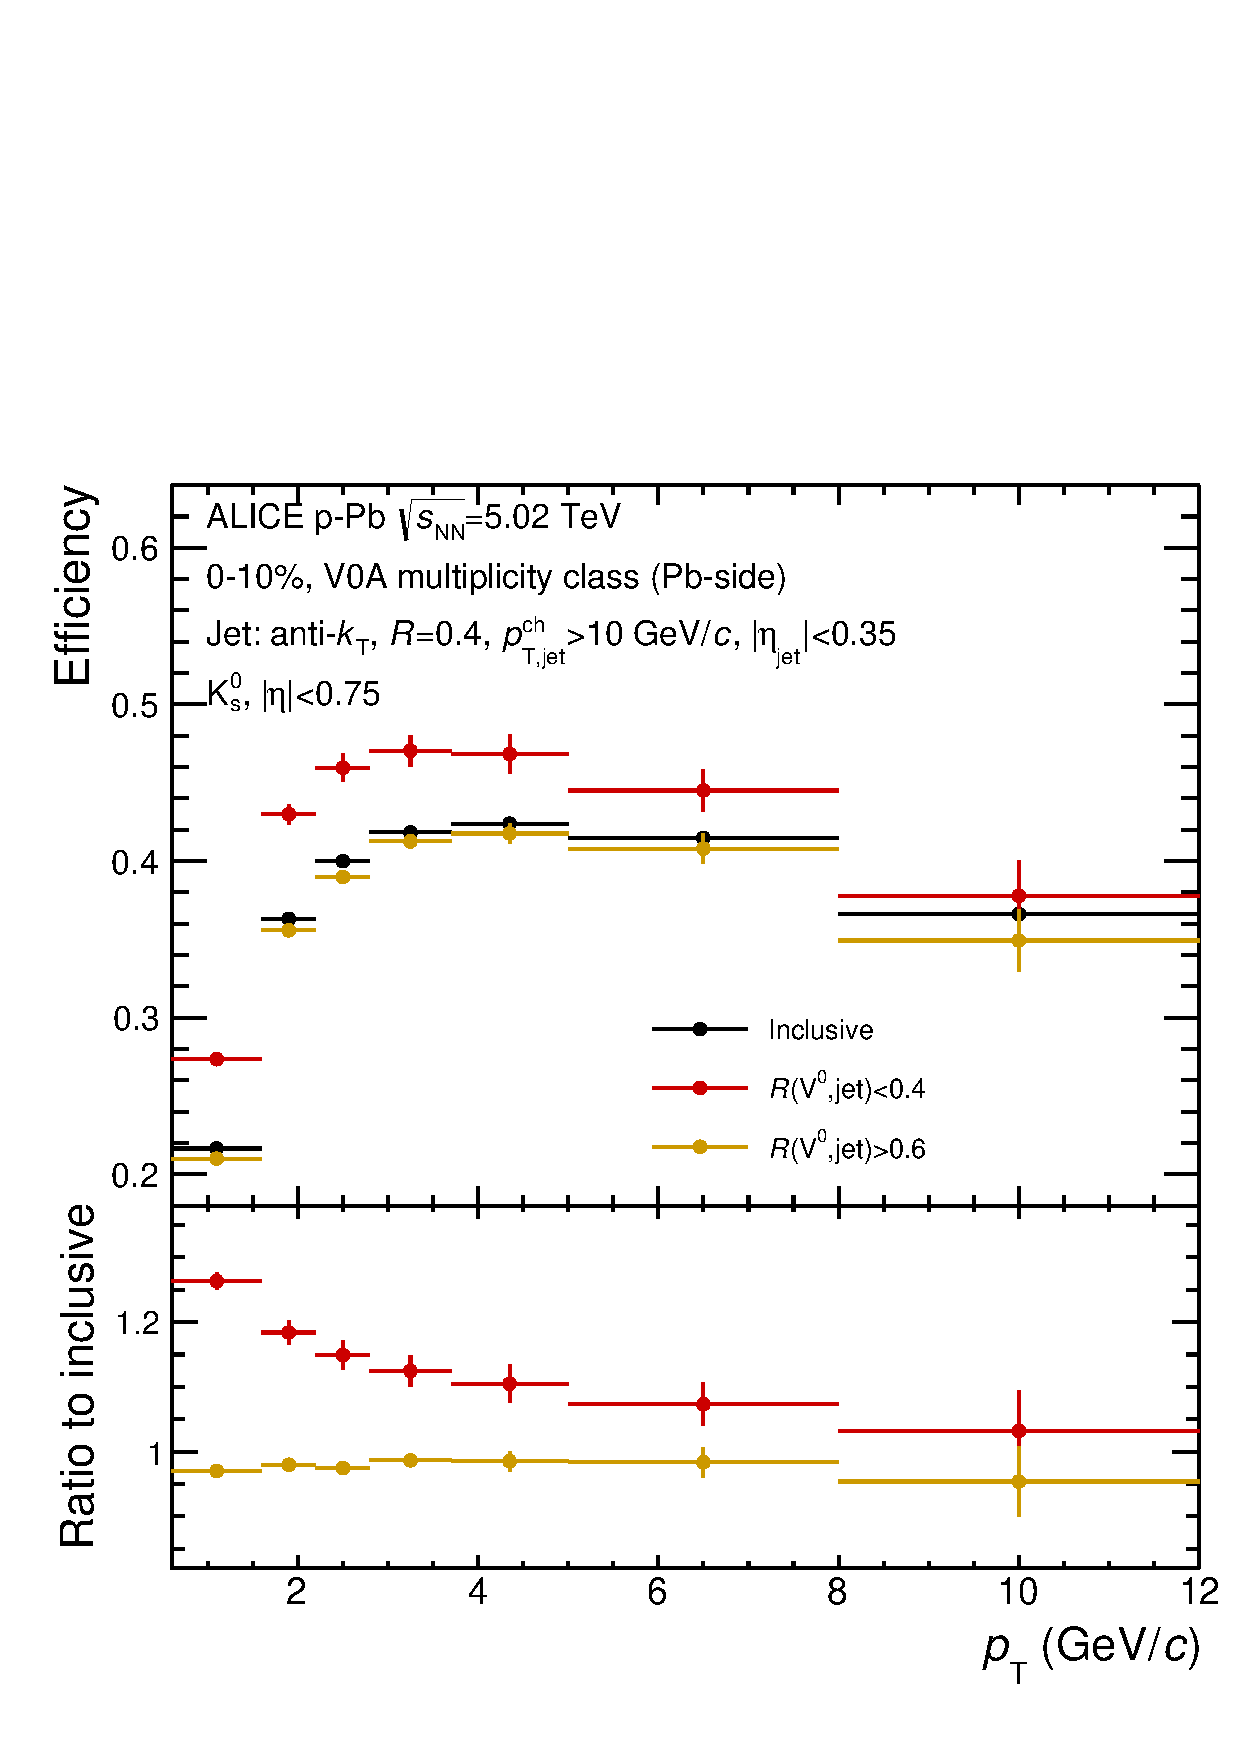
\includegraphics[width=.48\textwidth]{cEffiInJE_Kshort_JE_JR04_JC04_V0A_000_010}
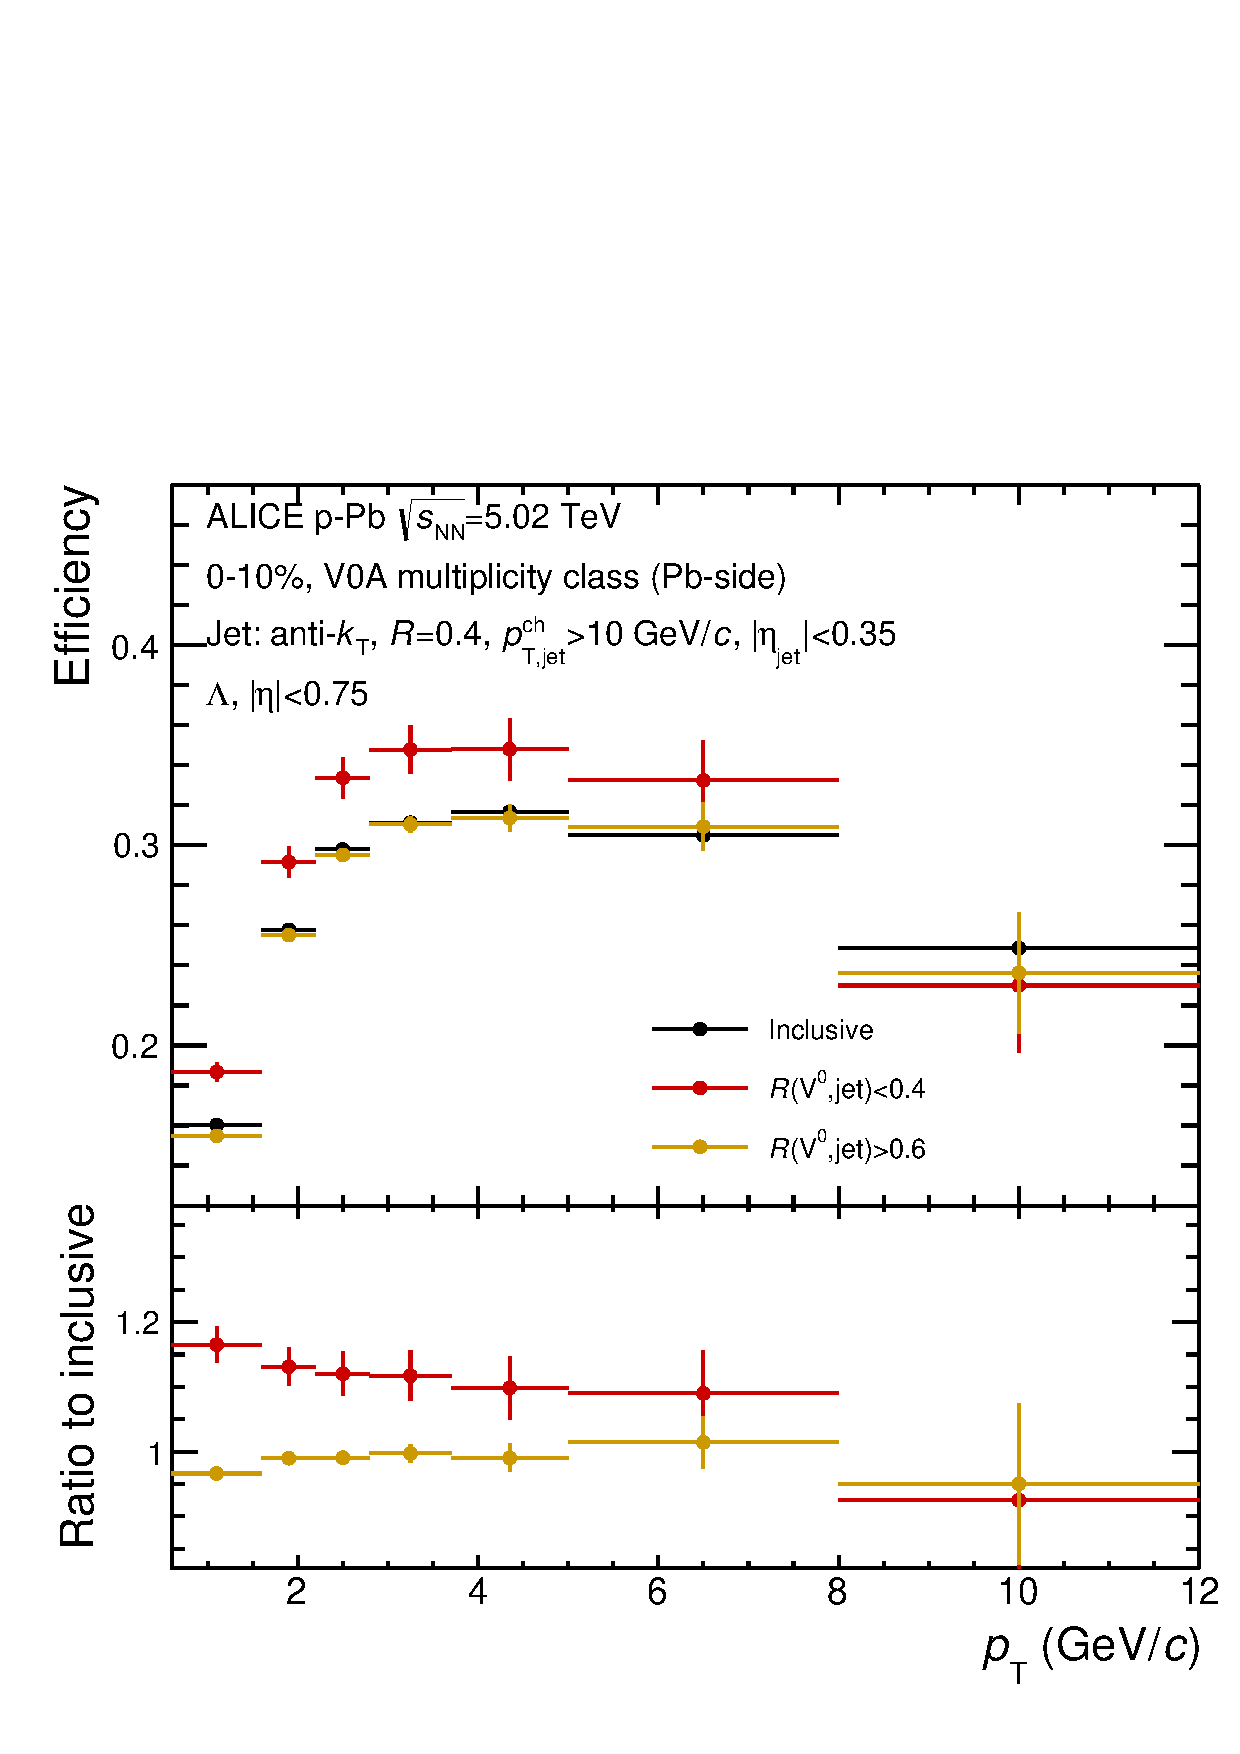
\includegraphics[width=.48\textwidth]{cEffiInJE_Lambda_JE_JR04_JC04_V0A_000_010}
\caption{Efficiency of inclusive $\Vzero$s as a function of $\pT$ \ask{(to be replaced by the MB ones)}.}
\label{fig:c05EffiV0InJets}
\end{center}
\end{figure}

To obtain the contribution from underlying event (UE $\Vzero$s, not associated to the hard scatterings) to the yield of JC $\Vzero$s, several estimators have been investigated.
\begin{itemize}
\item The OC selection: the $\Vzero$ candidates those were not matched to any selected jet with $R(\Vzero,{\rm jet})>R_{\rm cut}$.
\item The PC selection: the $\Vzero$ candidates found in the cones in the perpendicular directions of the selected jets \ask{(Add the PC definition explicitly? -- four PC cones are used)}.
\item The NJ selection: the $\Vzero$ candidates found in events those do not contain any jet with $\pT[jet]>5~\GeVc$.
\end{itemize}
The yields of different UE selections are extracted via the same approach as the JC $\Vzero$s.
The efficiency of OC $\Vzero$s with $R_{\rm cut}=0.6$ and $\pT[jet]>10~\GeVc$ is compared to those of inclusive $\Vzero$s and JC $\Vzero$s in figure~\ref{fig:c05EffiV0InJets}.
The efficiency of OC $\Vzero$s is similar to the inclusive $\Vzero$s and only a few precent lower than the inclusive one at low $\pT$.

\begin{figure}[t]
\begin{center}
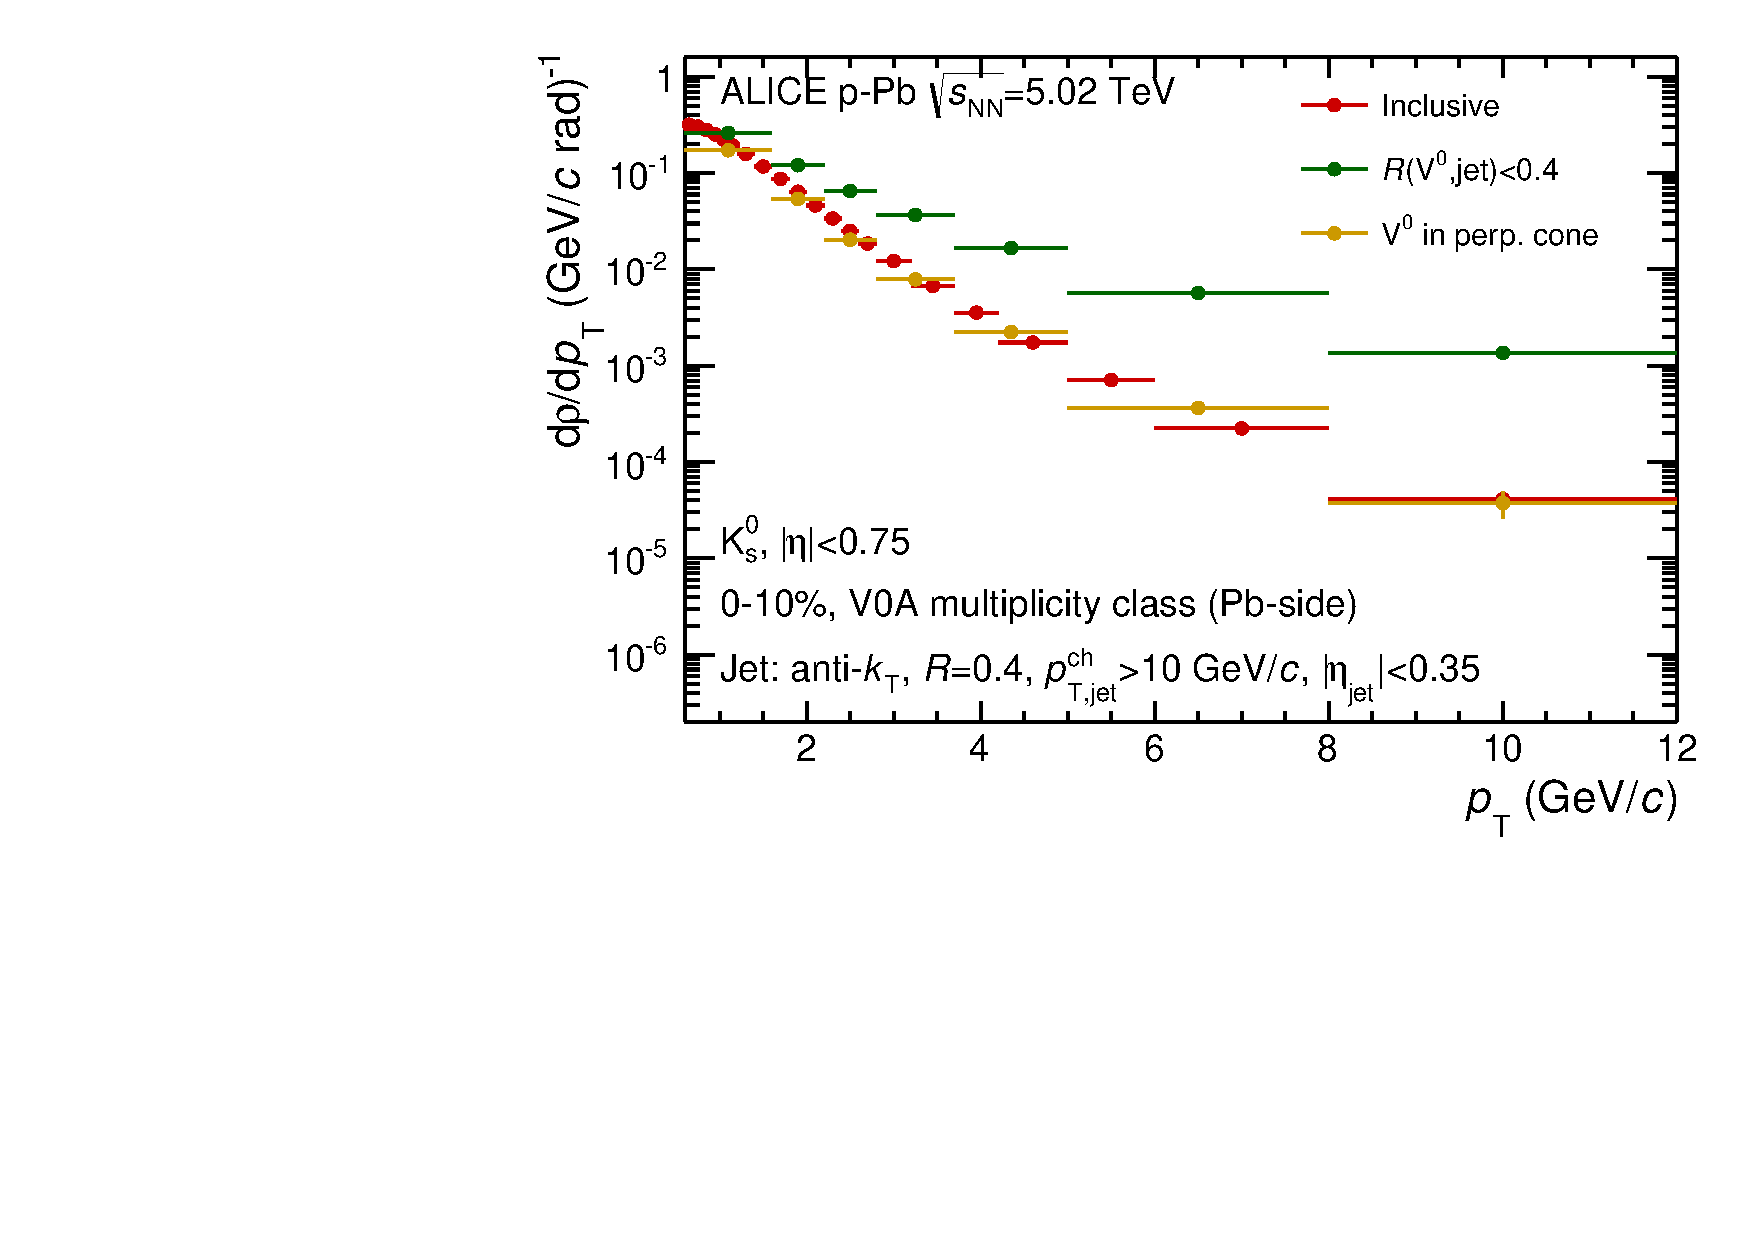
\includegraphics[width=.48\textwidth]{cRho_Kshort_JE_JR04_JC04_V0A_000_010}
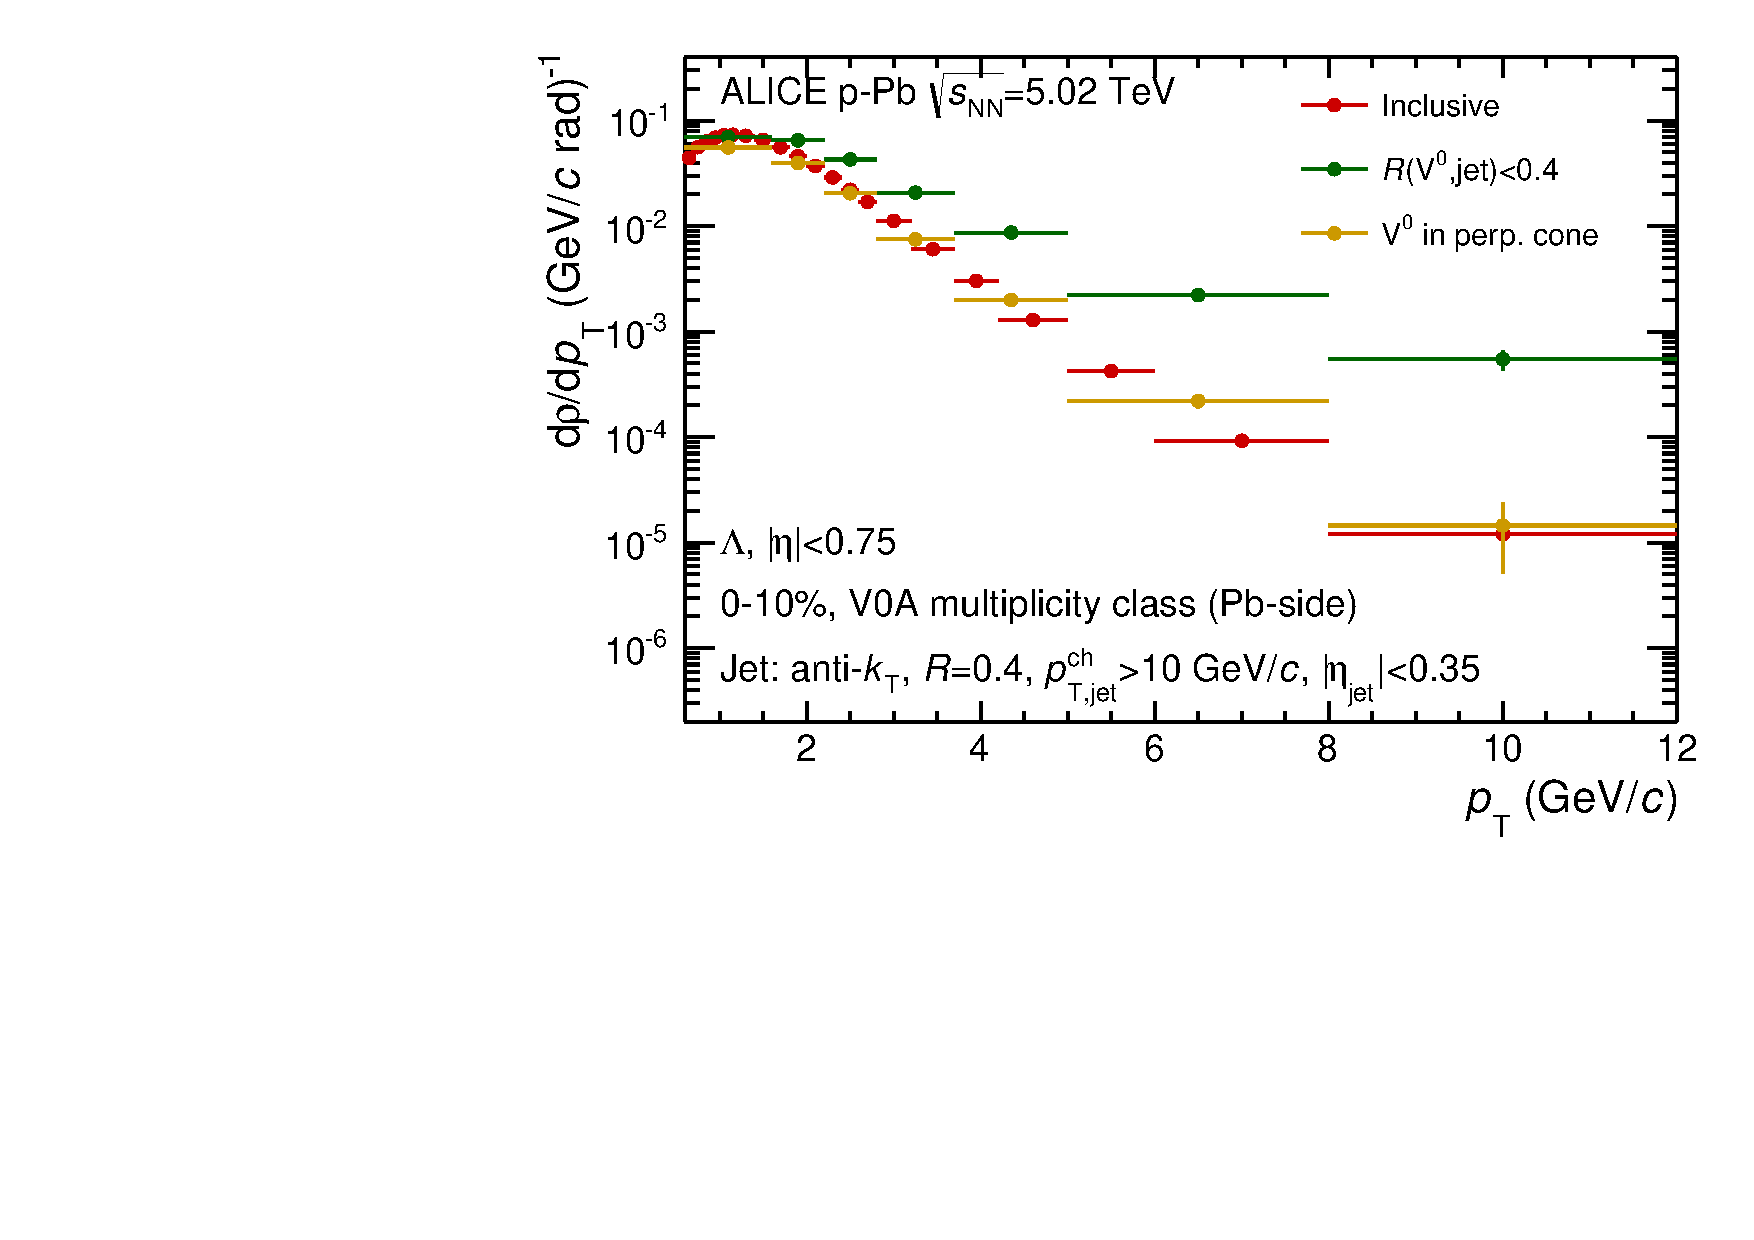
\includegraphics[width=.48\textwidth]{cRho_Lambda_JE_JR04_JC04_V0A_000_010}
\caption{$\pT$-differential density of $\Vzero$s in different selections \ask{(to be replaced by the MB ones)}.}
\label{fig:c05SpecV0s}
\end{center}
\end{figure}

Finally, to subtract the UE contribution from the JC selection, the efficiency corrected spectra of JC $\Vzero$s and UE $\Vzero$s have been normalized to the density per unit area,
\begin{equation}
\frac{\dd\rho_{\Vzero}}{\dd\pT}=\frac{1}{N_{\rm ev}}~\frac{1}{\avg{A_{\Vzero}}}~\frac{\dd N_{\Vzero}}{\dd\pT},
\end{equation}
where is $\avg{A_{\Vzero}}$ is the average acceptance for a given $\Vzero$ selection in $\hlab$--$\varphi$ plane calculated on a event-by-event basis.
Figure~\ref{fig:c05SpecV0s} shows the $\pT$-differential density distribution of inclusive $\Vzero$s and the JC and PC selections.
The $\pT$-differential density distribution of JC $\Vzero$s is much harder than those of inclusive $\Vzero$s and UE $\Vzero$s.
The density of $\Vzero$s associated to the hard scatterings, therefore, is obtained subtracting the density of UE $\Vzero$s from the JC selections.
\ask{More statements are needed -- (?)}
